
% FILE: figures/theory_graph.tex
% Graph of theories in K9

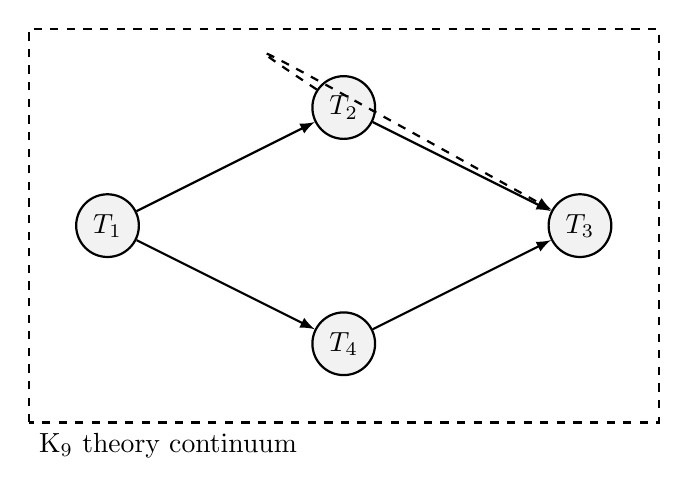
\begin{tikzpicture}[>=latex,thick,scale=1]
  % Theory nodes
  \node[draw, circle, fill=gray!10] (T1) at (0,0) {$T_1$};
  \node[draw, circle, fill=gray!10] (T2) at (3,1.5) {$T_2$};
  \node[draw, circle, fill=gray!10] (T3) at (6,0) {$T_3$};
  \node[draw, circle, fill=gray!10] (T4) at (3,-1.5) {$T_4$};

  % Edges
  \draw[->] (T1) -- (T2);
  \draw[->] (T2) -- (T3);
  \draw[->] (T1) -- (T4);
  \draw[->] (T4) -- (T3);
  \draw[dashed,->] (T2) .. controls (1.5,2.5) .. (T3);

  % Zones
  \draw[dashed] (-1.0,-2.5) rectangle (7.0,2.5);
  \node[anchor=north west] at (-1.0,-2.5) {K$_9$ theory continuum};
\end{tikzpicture}

